% -*- TeX-master: "ijcai18.tex" -*-

\section{Motivating example}\label{sec:example}

In this section, we give some background information on the Kappa
modelling language and introduce a toy example that motivates the need
for counterfactual reasoning in analyzing the causal structure of
simulationt traces.

% Maybe we should say a few eords here about what the model is about
% so that the reader is not shocked by the use of the word
% phosphorylation"


\subsection{Some background on Kappa}

In Kappa, proteins and other organic molecules are modelled by
abstract \emph{agents} with distinguishable \emph{sites}. Agents can
bind to each other through these sites and some sites also hold an
internal state. A site can only be engaged in at most one bond at a
time. The number and the nature of the sites featured by an agent
depend on its \emph{type}.
% , each type of agent being described in the model's
% \emph{signature}.
In our running example, there are two types of agents: substrates $S$
and kinases $K$. Agents of both type feature a binding site and a
phosphorylation site with two possible internal states:
\emph{unphosphorylated} and \emph{phosphorylated}.\footnote{Many
  proteins can be turned on and off by attaching or removing phosphate
  groups to some of their residues. The action of attaching a
  phosphate group to a protein is called phosphorylation and an enzyme
  catalyzing a phosphorylation reaction is called a kinase.}

We call \emph{mixture} a multiset of agents for which the internal
state and binding state of every site is fully specified.  Individual
agents are given global identifiers so that we can refer to them
unambiguously. \begin{figure}[!h]
  \vskip -0.25cm
  \begin{center}
    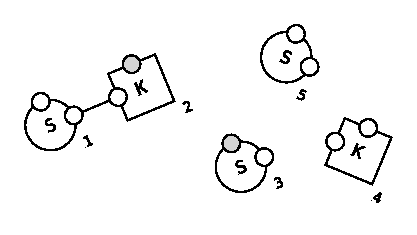
\includegraphics[scale=0.9]{figures/mixture.pdf}
  \end{center}
  \vskip -0.5cm
  \caption{An example of a reaction mixture. Instead of naming sites,
    we here identify them by their position on agents (phosphorylation
    sites are always shown on top). The relative position of agents in
    the figure is insignificant.  Phosphorylated sites are shown in
    gray.  Number labels correspond to global agent identifiers. }
  \label{fig:mixture}
\end{figure}

\noindent
Chemical interactions between agents are modelled by local
mixture-rewriting \emph{rules}.  A rule $r$ is defined by a triple
$(\RLHS{r}, \RRHS{r}, \lambda_r)$ that consists in a left-hand side, a
right-hand side and a firing rate.  Together, the rules of a model
denote a continuous-time Markov chain where
\begin{inparaenum}[(i)]
\item states are mixtures and
\item for every rule $r$, any part of the current mixture that matches
  $L_r$ is rewritten into $\RRHS{r}$ at rate $\lambda_r$.
\end{inparaenum}
Agents in our example model are subject to the set of rules depicted
in Figure~\ref{fig:model}. As expressed by these rules, kinases and
substrates can bind to each other provided that their respective
binding sites are free (rule ``$b$''). However, the resulting complex
is very unstable unless the kinase involved is phosphorylated, which
we model by introducing two unbind rules (``$u$'' and ``$u^{*}$'')
with different rates. Also, a substrate can get phosphorylated when it
is bound to a kinase (rule ``$p$''). Finally, for the sake of
simplicity, we model the phosphorylation process of kinases as a
spontaneous process (rule ``$pk$'').

% -*- TeX-master: "ijcai18.tex" -*-

\begin{figure}[h]
  \vskip -0.2cm
  \begin{center}
    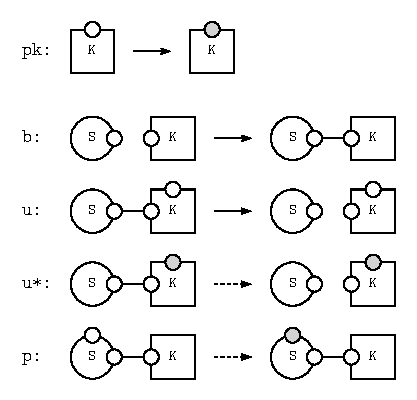
\includegraphics[scale=0.9]{figures/model.pdf}
  \end{center}
  \vskip -0.2cm
  % \caption{A motivating toy model. As usual in Kappa, sites not
  %   mentioned in a rule are left unchanged by it. Instead of naming
  %   sites, we here identify them by their position on an
  %   agent. Phosphorylated sites are shown in gray. Firing rates are
  %   not specified here but dotted arrows indicate \textit{slow}
  %   reactions, whereas solid arrows indicate \textit{fast} reactions.}
  \caption{A motivating toy model. Sites not mentioned in a rule are
    left unchanged by it. \longversion{As in
      Figure~\protect\ref{fig:mixture}, sites are identified by their
      position on an agent.}  Firing rates are not specified, but
    dotted (solid) arrows indicate \textit{slow} (\textit{fast})
    reactions
    $(\lambda_u \gg \lambda_{u^*} \approx \lambda_p)$.}
  \label{fig:model}
\end{figure}


Importantly, not every site of an agent has to be mentioned in a rule.
Following the \textit{``don't care, don't write"} principle, sites not
mentioned in a rule are left unchanged by it. Although this may appear
trivial, this is a defining feature of rule-based models, contrasting
with other modelling frameworks %that are frequently used in biology
like Petri-nets and differential equations where the chemical species
involved in a reaction have to be fully specified. The most obvious
benefit of the rule-based approach is that it enables a concise and
scalable representation of complex chemical systems that can generate
a combinatorial number of distinct species. More significantly for our
purposes though, it is especially suitable for causal analysis as it
does not obfuscate the causal structure of a system with irrelevant
context information, ideally enabling a one-to-one correspondence
between rules and elementary physical mechanisms.

A \emph{rule instance}, also called \emph{abstract event}, is a pair
$(r, \xi)$ where $r$ is a rule and $\xi$ maps the agents featured in
$\RLHS{r}$ to global agent identifiers. We say that $(r, \xi)$ is
\emph{triggerable} in mixture $m$ if the codomain of $\xi$ in $m$
matches $L_r$. In this case, we write $\TRIGGERABLE{m}{(r, \xi)}$ and
$\xi$ is called an \emph{embedding} of $L_r$ into $m$:
\[\EMBS{r}{m} \eqdef \{ \xi \,:\, \TRIGGERABLE{m}{(r, \xi)}\}.\]
Whenever $m \vdash (r, \xi)$, we write $\UPDATE{m}{(r, \xi)}$ the
mixture we get from $m$ by triggering rule instance $(r, \xi)$, which
is done by rewriting the codomain of $\xi$ into $\RRHS{r}$.  Finally,
in a given mixture $m$, the \emph{activity} of a rule $r$ is defined
as the product $\lambda_r|\EMBS{r}{M}|$ of its reaction rate by the
number of embeddings of $L_r$ into $m$. For example, in
Figure~\ref{fig:mixture}, rule $b$ has activity $2\lambda_b$ and rule
$u$ has activity $0$. The \emph{total activity} of a mixture is
defined as the sum of the activities of every rule.

Given an initial mixture, the continuous Markov chain underlying a
Kappa model can be simulated using the so-called \emph{Gillespie
  algorithm} \cite{DanosEtAl-APLAS07} that is depicted
Algorithm~\ref{alg:gillespie} and which consists in repeating the
following steps:
\begin{inparaenum}[(1)]
\item draw the timespan before the next simulation event from an
  exponential distribution of parameter the total activity of the
  mixture and increment the current time by this amount,
\item draw a rule $r$ with probability proportional to its activity
  and
\item pick uniformly an embedding $\xi$ of the left-hand side of $r$
  in $m$ and trigger abstract event $(r, \xi)$.
\end{inparaenum}
The Gillespie algorithm outputs a sequence of \emph{events}, an event
being formally defined as a pair $(e, t)$ where $e$ is an abstract
event and $t$ its time of happening. Such a sequence of events is
called a \emph{trace}.

\begin{algorithm}
\caption{Doob-Gillespie algorithm}\label{alg:gillespie}
\begin{spacing}{1.2}
\begin{algorithmic}
\vspace{0.2cm}
  \STATE $t \gets 0$
  \STATE $m \gets\ $ initial mixture
  \vspace{0.1cm}
  \WHILE{ $t < t_\text{\,end}$ }
      \vspace{0.1cm}
      \STATE $\alpha \gets \sum_r {\lambda_r |\EMBS{r}{m}|}$
      \vspace{0.1cm}
      \STATE draw $\delta \sim \textsc{Exp}(\alpha) $
      \STATE $t \gets t + \delta$
      \STATE draw a rule $r$ with probability
      $\propto \ \lambda_r |\EMBS{r}{m}|$
      \STATE draw an embedding $\xi$ uniformly in $\EMBS{r}{m}$
      %\STATE update $m$ by triggering event $((r, \xi), t)$
      \STATE $m \gets \UPDATE{m}{(r, \xi)}$
      \STATE log event $((r, \xi), t)$
  \ENDWHILE
\vspace{0.1cm}
\end{algorithmic}
\end{spacing}
\end{algorithm}

\noindent For a more rigorous account of Kappa's semantics, we refer
the reader to \cite{}.



\subsection{Where existing techniques fall short}

% What about asking the question for the specific trace to make it
% clearer we are talking about actual causality ?

Let's consider again our example model that is displayed
Figure~\ref{fig:model}.  For the sake of simplicity, consider an
initial mixture $I$ with only a single kinase and a single substrate
whose sites are free and unphosphorylated. We then ask: starting from
$I$, \textbf{how} is $p$ typically triggered ? We are not merely
looking for an account of reachability but rather for causal
narratives, that is, collections of necessary events connected by
causal influences.

A stochastic simulation might produce the following trace (events are
labelled by the rules that induced them):
\begin{align}\label{example-trace} b,\ \ u,\ \ pk,\ \ b,\ \ p,\ \
  u^{*},\ \ \cdots
\end{align} Figure~\ref{fig:dumb-story} depicts the causal narrative
explaining the occurrence of $p$ in this trace according to existing techniques
\cite{DBLP:conf/fsttcs/DanosFFHH12,DanosEtAl-CONCUR07}. The arrow
between $b$ and $p$ is called an \textit{activation arrow}, meaning
that $b$ modifies an aspect of state (by creating a link) that enables
$p$ to happen.\footnote{A more precise definition is given in section~\ref{sec:inhibition}.} In order to generate such a causal account, we first compute
a \emph{sub-trace} of (\ref{example-trace}) that is 
\begin{inparaenum}[(i)]
\item \emph{valid} in the sense that each of its events can be
  triggered in turn from the initial mixture and
\item \emph{minimal} in the sense that none of its strict valid
  sub-traces features $p$.
\end{inparaenum}
Then, we compute activation arrows within the resulting sub-trace so
as to obtain a directed acyclic graph whose nodes are events and whose
edges are activation arrows.

\begin{figure}[H]
  \vskip -0.8cm
  \begin{center}
    \includegraphics[scale=0.7]{figures/dot/dumb-story.pdf}
  \end{center}
  \vskip -1cm
  \caption{A causal explanation for $p$ in trace
    (\ref{example-trace}).  Events are labelled by the rules that
    induced them. The \emph{init} node corresponds to a special event
    that sets the mixture to its initial state.  }
  \label{fig:dumb-story}
\end{figure}


The narrative presented Figure~\ref{fig:dumb-story}, however, is blind
to the critical role of $pk$ in the original trace. Looking at the
rules in Figure~\ref{fig:model} one notes that:
\begin{inparaenum}[(i)]
\item the phosphorylation rule $p$ is slow
\item the average time $K$ and $S$ remain bound depends on whether $K$
  is phosphorylated, as manifest in the two unbinding rules $u$ (fast,
  if $K$ is not phosphorylated) and $u^{*}$ (slow, if $K$ is
  phosphorylated).
\end{inparaenum} It seems reasonable to assert that $p$ would probably
not have happened had $pk$ not happened, as the opportunity for $p$
would have been cut short by a fast unbinding event. We therefore
argue that $pk$, although it does not activate $b$ or $p$ directly,
should be part of a causal narrative for $p$. Reasoning of this kind
is \textit{counterfactual} and can be deployed to define causality
\cite{lewis1974causation,pearl2009causality}.

In section~\ref{sec:counterfactual}, we give a rigorous semantics to
this line of reasoning and introduce an algorithm for simulating
counterfactual scenarios. In section~\ref{sec:inhibition} we show that
counterfactual statements can be expressed using inhibition arrows,
leading to the explanation shown in Figure~\ref{fig:cex}.
